
\section{Improvements}
\label{sec:improvements}

While developing and testing the algorithm, 2 main obstacles prevented from using larger datasets and smaller minSupport:
\begin{enumerate}
	\item Memory - Tree size.
	\item Computation Time - Tree order.
\end{enumerate}

\subsection{IPFIM-Improved}
To handle these obstacles, 2 techniques were implemented.
To handle the computation time, an approach similar to CPTree~\ref{par:cptree} was tested, where we defined a semi-frequency order on 1st dataset half, and used it for the rest of the iterations. New items were sorted canonically.

To handle the memory limitation, which is caused by the construction of a large tree, a partial approach of ~\ref{par:AFPIM} was used - We added a pre-min support to identify pre-frequent items. For the simplicity of the experiment, items which where not frequent in iteration i, and will become frequent after sum of j iterations, are waived. A trade-off between missing items and tree size can be controlled using the pre-min parameter.  Also, as mentioned earlier, since we use a semi-frequent order similar to ~\ref{par:cptree}, no need to perform ~\ref{AFPIMAdjust}, only ~\ref{AFPIMRemove} and recalculation for items that are under case 4 in ~\ref{tab:AFPIMCases}.

The algorithm is presented in ~\autoref{alg:IPFIMImprovedIteration}, the main change is in the $IPFIMImprovedIteration$ method on lines 2:3, where we first update the global frequency list and clear the items below minMinSupport before adding the transaction to the trees.

\begin{algorithm}
  \caption{IPFIMImprovedIteration}
  \begin{algorithmic}[1]
   \label{alg:IPFIMImprovedIteration}
    \Procedure{IPFIMImprovedIteration}{data,canTrees,sortFunction,partitioner,minMinSup,freqList}
    \State $freqList\gets\text{update with data count}$
    \State $filteredData\gets\text{filter from data where itemCount<minMinSup }$
    \State $sortedAndFilteredTransactions\gets\text{order filteredData by sortFunction}$
    \State $partitionedTransactions\gets\text{map sortedAndFilteredTransactions to key'=g; value'={t\textsubscript{i}[0]…t\textsubscript{i}[L]}}$ \Comment{As in PFP}
	\State $canTrees \gets\text{Reduce partitionedTransactions and update trees}$
	\State \textbf{return} $canTrees$
    \EndProcedure
  \end{algorithmic}
\end{algorithm}


%\subsection{IPFIM Improved vs IPFIM - Computation}
%Although the size of the tree was not effected by more than 10\%, when using semi-frequency order, computation time was improved by ~30X when running single partition, as seen in \autoref{fig:partialcannonical}.
%%\begin{figure}
%%  \centering
%%  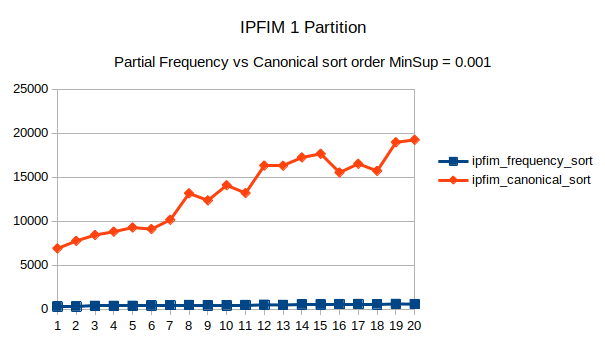
\includegraphics[width=\linewidth]{figures/ipfim_freq_vs_can_sort}
%%  \caption{IPFIM partial frequency sort vs IPFIM cannonical sort}
%%  \label{fig:partialcannonical}
%%\end{figure}
%
%\subsection{IPFIM Improved vs IPFIM - Memory}
%Using a partial approach of AFPIM~\cite{koh2004efficient}, we were able to run synthetic datasets of 100M transactions and 100k unique item sets. The results, compared to PFP, for 100 partitions, min support of 0.01 and 0.003 can be seen  in \autoref{fig:ipfimImpT20}. As there is only 1 dataset scan for IPFIM, and we pre-defined the semi-frequency order, the results are 10x faster even for 1st iteration, and improve to 25x for last one.
%
%%\begin{figure}
%%  \centering
%%  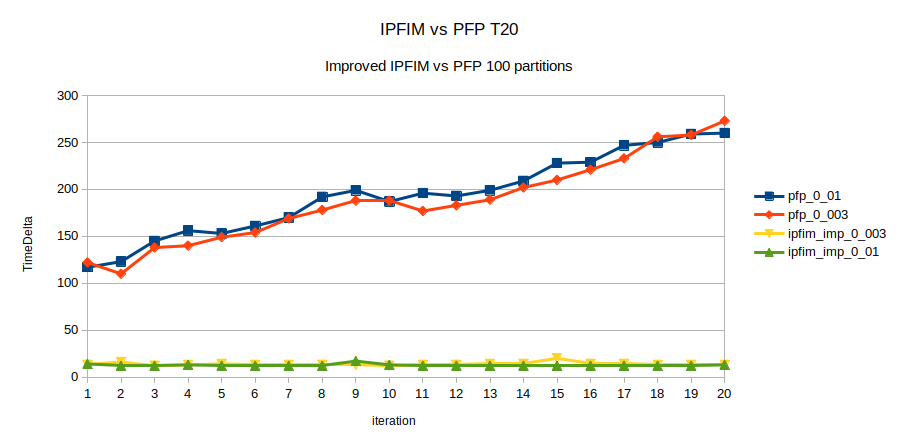
\includegraphics[width=\linewidth]{figures/t20_ipfim_imp_vs_pfp}
%%  \caption{IPFIM pre-min, semi-frequency vs PFP}
%%  \label{fig:ipfimImpT20}
%%\end{figure}
